\documentclass{rosenpass-beamer}

\usepackage[german]{babel}
\usepackage[autostyle]{csquotes}
\usepackage{emoji}
%\usepackage{dirtytalk}
\let\say\enquote

\usepackage{xurl}

\urlstyle{same}

\usepackage{textcomp}

\usetikzlibrary{positioning,decorations.pathreplacing,svg.path}

\definecolor{RPPink}{rgb}{274,4,132}
\definecolor{RPOrange}{rgb}{255, 166, 48}
\definecolor{RPAquamarine}{rgb}{255, 166, 48}
\definecolor{RPLightGray}{rgb}{160, 159, 164}
\definecolor{RPTurquoise}{rgb}{114, 161, 229}

\title{Rosenpass}
\subtitle{VPN \& Struktur für Translationsforschung in der Kryptografie}
\author{
Wanja Zaeske, Stephan Ajuvo, Marei Peischl, Benjamin Lipp, Lisa~Schmidt, Karolin Varner
}
\institute{\url{https://rosenpass.eu}}


\conference{IAV – Regelrunde Embedded Security}
\date{2023-07-03}

\parskip\smallskipamount

% reduce itemize indent
\setlength{\leftmargini}{0pt}

\usepackage{biblatex}
\addbibresource{sources.bib}

\graphicspath{{}{graphics/}}

\begin{document}

\maketitle

\begin{frame}{Das Rosenpass-Projekt}
\begin{columns}[c,onlytextwidth]
\begin{column}{.6\textwidth}
\begin{itemize}
  \item Quantencomputer-sichere Kryptografie
  \item Forschung
  \item Ergebnisse in die Anwendung bringen
  \item Zusammenarbeit mit Industrie
\end{itemize}
\end{column}
\begin{column}{.4\textwidth}
\centering
  \includegraphics[width=\linewidth]{graphics/qc.png}
\end{column}
\end{columns}
\end{frame}

\begin{frame}{Warum sind Quantencomputer (k)eine Bedrohung?}
\begin{columns}[b]
\begin{column}{.75\textwidth}
\begin{itemize}
  \item Grovers Algorithmus \strong{schwächt} symmetrische Kryptografie
  \begin{itemize}
    \item AES, SHA-2, SHA-3, Chacha20
    \item Lösung: größere Keys
  \end{itemize}
  \item Shors Algorithmus \strong{bricht} asymmetrische Kryptografie
  \begin{itemize}
    \item RSA, DSA, DH, ECDH
    \item Lösung: alternative Kryptografie
  \end{itemize}
  \item  Nur auf großen Quantencomputern
  \begin{itemize}
    \item Die existieren noch nicht
    \item Problem: Store now, decrypt later
  \end{itemize}
\end{itemize}
\end{column}
\begin{column}{.25\textwidth}
\makebox[\linewidth][r]{%
\includegraphics[width=1.5\linewidth]{graphics/qc and crypto.png}
}%
\par
\imgNote{\makebox[\linewidth][r]{Quantencomputer überschatten Kryptografieverfahren.}}
\end{column}
\end{columns}
\end{frame}

\begin{frame}{Sichere Kommunikation durch VPN}
\begin{columns}[T]
\begin{column}{0.5\textwidth}
%\begin{block}{Traffic durch VPN}
\begin{itemize}
\item  Ermöglicht Sicherheit ohne Anpassung von Applikationen
\item  Protokoll: WireGuard \raisebox{\dimexpr-.5\height+.5\ht\strutbox}[0pt][0pt]{\includegraphics[height=1.5\baselineskip]{graphics/wireguard}}

  \begin{itemize}
    \item Schnell
  \item Effizient
  \item Open Source
  \item Kompatibel
  \item Etabliert
  \item Problem: nutzt ECDH, also angreifbar!
  \end{itemize}
\end{itemize}
%\end{block}
\end{column}

\begin{column}{0.4\textwidth}
\includegraphics[width=\textwidth]{graphics/qc and crypto.png}

\imgNote{Quantencomputer überschatten Kryptografieverfahren.}

\end{column}
\end{columns}
\end{frame}

\begin{frame}{Wie löst Rosenpass das Problem?}
\begin{itemize}
\item  Basiert auf PQ-sicherer asymmetrisch Kryptografie

  \begin{itemize}
  \item Classic McEliece
  \item Kyber
  \end{itemize}
\item  Benötigt: Public Key von anderen Peers
\item  Erzeugt: Shared Secrets zwischen Peers
\item  Angriff mit Quantencomputer nicht effizient
\item  Rosenpass, das Protokoll

  \begin{itemize}
    \item Nutzt 3-Way Handshake
  \item Secret wird alle 2 Minuten rotiert
  \item Authentication, Secrecy und Integrity
  \end{itemize}
\end{itemize}
\end{frame}

\begin{frame}{PQ-sichere Kommunikation: WireGuard + Rosenpass}
\begin{itemize}
\item  Hybride Sicherheit

  \begin{itemize}
    \item Bricht nur, wenn Rosenpass \textbf{und} WireGuard versagen
  \end{itemize}
\item  Überall nutzbar, wo WireGuard schon läuft
\item  Ohne Anpassung vom WireGuard Source Code

  \begin{itemize}
    \item Shared Secret aus Rosenpass = PSK für WireGuard
  \end{itemize}
\item  Aber:

  \begin{itemize}
    \item Ein Prozess mehr
  \item Handshake alle 2 Minuten
  \end{itemize}
\end{itemize}

\makebox[\linewidth][c]{%
\includegraphics[width=.6\linewidth]{graphics/wireguard and rp.png}}

\imgNote{\makebox[\linewidth][c]{WireGuard mit Rosenpass.}}
\end{frame}

\begin{frame}{Rosenpass Struktur}
\begin{columns}[c]
\begin{column}{0.7\textwidth}
\begin{itemize}
\item  Zusammenkunft von Kryptografie, Dev und SciComm Experten
\item  Idee: Team festigen
\item  Mittel: Rosenpass e.\,V.

  \begin{itemize}
    \item Zusammenarbeit mit Industrie
  \item Ansprechpartner für Integratoren
  \end{itemize}
\item  Rosenpass Roadmap

  \begin{itemize}
    \item Rosenpass in Embedded
  \item Rosenpass in Datacenter
  \item Integration in andere Apps
  \end{itemize}
\item  Kryptografie + Safety Forschung

  \begin{itemize}
    \item Decryption Despite Error
  \end{itemize}
\end{itemize}
\end{column}

\begin{column}{0.2\textwidth}
\includegraphics[width=\linewidth]{graphics/rosenpass in anderen apps.png}

\medskip
\includegraphics[width=\linewidth]{graphics/Illu-install.png}

\imgNote{Anwendungsfälle.}
\end{column}
\end{columns}
\end{frame}


\end{document}

%%%%%%%%%%%%%%%%%%%%%%%%%%%%%%%%%%%%%%%%%%%%%%%%%%%%%%%%%%%%
% Wozu braucht es Post-Quantum Krypto

\begin{frame}{Angriffe von Quantencomputern: Shors\footnote{Peter Shor} Algorithmus}

\textbf{Jargon}: Löst einige mathematische Probleme effizient, auf denen moderne Krypto basiert:

%\vspace{5mm}



\begin{itemize}
    \item RSA\footnote{\say{Rivest-Shamir-Adleman} -- Ron Rivest, Adi Shamir, Leonard Adleman} (das \emph{Faktorisierungsproblem} – Primzahlzerlegung)
    \item DH\footnote{\say{Diffie-Hellmann} -- Whitfield Diffie, Martin Hellmann} (Berechnen des \emph{Diskreten Logarithmus})
    \item ECDH\footnote{Elliptic Curve Diffie-Hellmann} (Berechnen des \emph{Diskreten Logarithmus auf Elliptischen Kurven})
\end{itemize}

%\vspace{5mm}

\textbf{Weniger Jargon}: Bricht so ziemlich alle moderne, asymmetrische Kryptographie.

\end{frame}

\begin{frame}{Angriffe von Quantencomputern: Grovers\footnote{Lov Grover} Algorithmus}

\textbf{Jargon}: Suche durch ungeordnete Listen in $O(\sqrt{n})$ statt klassisch $O(n)$ im Durchschnitt.

\vspace{5mm}


\textbf{Weniger Jargon}: Mostly harmless (\say{im wesentlichen harmlos});\\
symmetrische Kryptographie ist kaum betroffen.

\end{frame}

\begin{frame}{Quantencomputer: Ein ganz heißes Eisen}
  \ImgSource{\includegraphics[height=.8\textheight]{assets/xkcd_678.png}}{https://xkcd.com/678/}
\end{frame}

\begin{frame}{Post-Quanten-Kryptographie: Munch now decrypt later}
\begin{columns}[c]
\column{.6\textwidth}
\begin{itemize}
    \item Post-Quanten-Kryptographie ist auf dem Weg der Standardisierung
    \item Wir müssen sehr früh deployen;\\
    wenn die Krypto kaputt ist, dann ist es zu spät.
\end{itemize}
\column{.4\textwidth}
\ImgSource{%
\makebox[\linewidth][c]{
  \includegraphics[height=.5\textheight]{assets/gray-hamster-eating-sunflower-seed.jpeg}}}{%
   \url{https://foto.wuestenigel.com/gray-hamster-eating-sunflower-seed/}}
  
  \say{Munch now decrypt later}\footnotemark
\end{columns}
\footnotetext{\say{Jetzt speichern später entschlüsseln}. Warnung: Geheimdienste sind nicht so cute wie dieser Hamster.}
\end{frame}

\begin{frame}{Post-Quanten-Kryptographie: Wird bereits standardisiert}

\begin{columns}[T]
\begin{column}{.50\textwidth}

\large Durch NIST\footnotemark zur Standardisierung ausgewählt \cite{nist-selected-algorithms}:
\normalsize

%\footnote{Quelle: https://csrc.nist.gov/Projects/post-quantum-cryptography/selected-algorithms-2022} \normalsize

\vspace{2mm}

\begin{itemize}
    \item Crystals-Kyber (Verschlüsselung)
    \item Crystals-Dilithium (Signatur)
    \item Falcon (Signatur)
    \item Sphincs+ (Signatur)
\end{itemize}

\end{column}
\footnotetext{National Institut for Standards and Technology – US-Amerikanische Standardisierungsbehörde} 

\begin{column}{.50\textwidth}
\large Das BSI\footnotemark empfiehlt \cite{bsi-quantensicher-gestalten}\normalsize:

\vspace{2mm}

\begin{itemize}
    \item Frodo (Verschlüsselung)
    \item Classic McEliece (Verschlüsselung)
\end{itemize}

\end{column}
\footnotetext{Bundesamt für Sicherheit in der Informationstechnik} 
\end{columns}

\end{frame}

\begin{frame}[label=NIKE]{Verschlüsselung im Angesicht von Quantencomputern}
    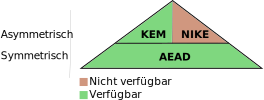
\includegraphics[height=.6\textheight]{graphics/Primitivenpyramide.pdf}
      
    Die meisten Schlüsselaustausch-Protokolle inklusive WireGuard nutzen NIKEs    
\end{frame}

%%%%%%%%%%%%%%%%%%%%%%%%%%%%%%%%%%%%%%%%%%%%%%%
% Rosenpass Demo

\begin{frame}{Rosenpass Demo!}
  \includegraphics[height=.9\textheight]{assets/2023-03-20-rg-tutorial-screenshot.png}
\end{frame}

%%%%%%%%%%%%%%%%%%%%%%%%%%%%%%%%%%%%%%%%%%%%%%%%
%% Wie funktioniert Rosenpass

\againframe{NIKE}

%\begin{frame}{naming scheme}
%\begin{block}{}
%	\begin{tikzpicture}
%		\namepart{s=Static,e=Ephemeral}
%		\namepart[2.2cm]{sk=Secret Key,pk=Public Key,pt=Plaintext,ct=Ciphertext}
%		\namepart[4.4cm]{i=Initiator,r=Responder,m=Mine,t=Theirs}
%		\begin{scope}[decoration={brace,amplitude=3mm},thick]
%			\namebraceright{s}{e}
%			\namebraceleft{sk}{ct}
%			\namebraceright{sk}{ct}
%			\namebraceleft{i}{t}
%		\end{scope}
%	\end{tikzpicture}
%\end{block}
%\end{frame}


\begin{frame}[b]{Schlüsselaustauschmethoden:}
\framesubtitle{Static-static Schlüsselaustausch mit NIKEs\footnote{\say{Non-Interactive Key Exchange} -- Nichtinteraktiver Schlüsselaustausch}}
\hspace*{-.9\csname beamer@leftmargin\endcsname}\begin{tikzpicture}[
rosenpass-diagram,
  % define multiple syles for consistency
  boxed-node/.style = {draw, rectangle, fill=white, text width = 5em, align = center, minimum height = 1.75em, rounded corners},
  swimming-lane/.style = {very thick},
  message-flow/.style = {-{Stealth[length = 0.5em]}, shorten >= 0.25em, shorten <= 0.25em},
  yscale=.7
]

  % iterate over i, multiply with 1cm, creating a vertical, down moving row of coordinates
  \foreach \i [evaluate=\i as \angle using { \i * 1cm}] in {0,...,5}
    \coordinate (n-\i) at (0,-\i);

  % set two initial nodes, positioned relative to the coordinates
	 \draw[initiator](-1,0) node(initiator){Initiator} coordinate(ini) ++(0,.1)to
		coordinate[pos=.2](spki-y)
		coordinate[pos=.6](spkr-y)
		coordinate[pos=.76](ack-y)+(0,-5) coordinate(result-y);
	  \draw[responder] (1,0) node(responder){Response} coordinate (res)++(0,.1)to +(0,-5);
%  \node[boxed-node] (ini) at (n-0) {Initiator};
%  \node[boxed-node,right = of ini] (res) {Response};

  % place a text on the intersection of the ini node and the n-1 coordinate
  \node[anchor = east] (sski) at (n-1 -| ini) {(sski, spki) $\leftarrow$ keygen()};

  % place a text on the intersection of the res node and the n-2 coordinate
  \node[anchor = west] (sskr) at (n-2 -| res) {(sskr, spkr) $\leftarrow$ keygen()};

  % place text on below ini and res node on the height of the n-3 coordinate
  \node[anchor = east] (dhi) at (n-4 -| ini) {key $\leftarrow$ dh(sski, spkr)};
  \node[anchor = west] (dhr) at (n-4 -| res) {key $\leftarrow$ dh(sskr, spki)};

  % TODO: Horizontale (gestrichelte) linie um zu zeigen wo das setup endet?

  % define the vertical swimming lanes
%  \begin{scope}[style = swimming-lane]
%     \draw (ini) -- (n-5 -| ini);
%     \draw (res) -- (n-5 -| res);
%  \end{scope}

  % define the message flows
  \begin{scope}[style = message-flow]
     \draw [request](sski) -- node[above]{spki} (sski -| res);
     \draw [response](n-2 -| ini) -- node[above]{spkr} (n-2 -| res);
  \end{scope}
\end{tikzpicture}\hfill\begingroup\footnotesize
\raisebox{-\baselineskip}{\makebox[4cm][l]{%
	\begin{tikzpicture}[outer sep=1mm]
		\namepart{s=Static,e=Ephemeral}
		\namepart[2cm]{sk=Secret Key,pk=Public Key,ct=Ciphertext}
		\namepart[4cm]{i=Initiator,r=Responder}
		\begin{scope}[decoration={brace,amplitude=3mm},thick]
			\namebraceright{s}{e}
			\namebraceleft{sk}{ct}
			\namebraceright{sk}{ct}
			\namebraceleft{i}{r}
		\end{scope}
\end{tikzpicture}}}
\endgroup
%Static-static Schlüsselaustausch mit NIKEs.
\end{frame}

%\end{document}
%
\begin{frame}[b]{Einfachst-möglicher Schlüsseltausch mit KEMs\footnote{\say{Key-Encapsulation Method} -- Schlüsseltransportmethode}}
\hspace*{-.9\csname beamer@leftmargin\endcsname}\begin{tikzpicture}[
rosenpass-diagram,
  % define multiple syles for consistency
  boxed-node/.style = {draw, rectangle, fill=white, text width = 5em, align = center, minimum height = 1.75em, rounded corners},
  swimming-lane/.style = {very thick},
  message-flow/.style = {-{Stealth[length = 0.5em]}, shorten >= 0.25em, shorten <= 0.25em},
  yscale=.8
]

  % iterate over i, multiply with 1cm, creating a vertical, down moving row of coordinates
  \foreach \i [evaluate=\i as \angle using { \i * .8cm}] in {0,...,6}
    \coordinate (n-\i) at (0,-\i);

  % set two initial nodes, positioned relative to the coordinates
		 \draw[initiator](-1,0) node(initiator){Initiator} coordinate(ini) ++(0,.1)to
			coordinate[pos=.2](spki-y)
			coordinate[pos=.6](spkr-y)
			coordinate[pos=.76](ack-y)+(0,-5) coordinate(result-y);
		  \draw[responder] (1,0) node(responder){Response} coordinate (res)++(0,.1)to +(0,-5);
	

  % place a text on the intersection of the res node and the n-2 coordinate
  \node[anchor = west] (sskr) at (n-1 -| res) {(sskr, spkr) $\leftarrow$ keygen()};

  % place a text on the intersection of the res node and the n-2 coordinate
  \node[anchor = east] (sctr) at (n-3 -| ini) {(key, sctr) $\leftarrow$ encaps(spkr)};
  \node[anchor = west] (decapsr) at (n-3 -| res) {key $\leftarrow$ decaps(sctr)};

  % define the vertical swimming lanes
%  \begin{scope}[style = swimming-lane]
%     \draw (ini) -- (n-6 -| ini);
%     \draw (res) -- (n-6 -| res);
%  \end{scope}

  % define the message flows
  \begin{scope}[style = message-flow]
     \draw [response](n-1 -| ini) -> node[above]{spkr} (n-1 -| res);
     \draw [request](sctr) -> node[above]{sctr} (sctr -| res);
  \end{scope}
\end{tikzpicture}%
\hfill
\begingroup\footnotesize
\raisebox{-\baselineskip}{%
\makebox[4cm][l]{%
	\begin{tikzpicture}[outer sep=1mm]
		\namepart{s=Static,e=Ephemeral}
		\namepart[2cm]{sk=Secret Key,pk=Public Key,ct=Ciphertext}
		\namepart[4cm]{i=Initiator,r=Responder}
		\begin{scope}[decoration={brace,amplitude=3mm},thick]
			\namebraceright{s}{e}
			\namebraceleft{sk}{ct}
			\namebraceright{sk}{ct}
			\namebraceleft{i}{r}
		\end{scope}
\end{tikzpicture}}}
\endgroup
\end{frame}
\begin{frame}{Schlüsselaustauschmethoden:}
\framesubtitle{Mit KEMs
%\footnote{\say{Key-Encapsulation Method} -- Schlüsseltransportmethode}
wird es komplizierter}
\begin{tikzpicture}[
rosenpass-diagram,
  % define multiple syles for consistency
  boxed-node/.style = {draw, rectangle, fill=white, text width = 5em, align = center, minimum height = 1.75em, rounded corners},
  swimming-lane/.style = {very thick},
  message-flow/.style = {-{Stealth[length = 0.5em]}, shorten >= 0.25em, shorten <= 0.25em},
  yscale=.8
]

  % iterate over i, multiply with 1cm, creating a vertical, down moving row of coordinates
  \foreach \i [evaluate=\i as \angle using { \i * .8cm}] in {0,...,6}
    \coordinate (n-\i) at (0,-\i);

  % set two initial nodes, positioned relative to the coordinates
%  \node[boxed-node] (ini) at (n-0) {Initiator};
%  \node[boxed-node,right = of ini] (res) {Response};
	 \draw[initiator](-1,0) node(initiator){Initiator} coordinate(ini) ++(0,.1)to
		coordinate[pos=.2](spki-y)
		coordinate[pos=.6](spkr-y)
		coordinate[pos=.76](ack-y)+(0,-5) coordinate(result-y);
	  \draw[responder] (1,0) node(responder){Response} coordinate (res)++(0,.1)to +(0,-5);

  % place a text on the intersection of the ini node and the n-1 coordinate
  \node[anchor = east] (sski) at (n-1 -| ini) {(sski, spki) $\leftarrow$ keygen()};

  % place a text on the intersection of the res node and the n-2 coordinate
  \node[anchor = west] (sskr) at (n-2 -| res) {(sskr, spkr) $\leftarrow$ keygen()};

  % place a text on the intersection of the res node and the n-2 coordinate
  \node[anchor = east] (sctr) at (n-4 -| ini) {(key1, sctr) $\leftarrow$ encaps(spkr)};
  \node[anchor = west] (decapsr) at (n-4 -| res) {key1 $\leftarrow$ decaps(sctr)};

  \node[anchor = west] (scti) at (n-5 -| res) {(key2, scti) $\leftarrow$ encaps(spki)};
  \node[anchor = east] (decapsi) at (n-5 -| ini) {key2 $\leftarrow$ decaps(scti)};

  % define the vertical swimming lanes
%  \begin{scope}[style = swimming-lane]
%     \draw (ini) -- (n-6 -| ini);
%     \draw (res) -- (n-6 -| res);
%  \end{scope}

  % define the message flows
  \begin{scope}[style = message-flow]
     \draw[request] (sski) -> node[above]{spki} (sski -| res);
     \draw[response]  (n-2 -| ini)-> node[above]{spkr} (n-2 -| res);

     \draw[request] (sctr) -> node[above]{sctr} (sctr -| res);
     \draw [response] (n-5 -| ini)   -> node[above]{scti}  (n-5 -| res);
  \end{scope}
\end{tikzpicture}

Static-static Schlüsselaustausch mit KEMs.

\end{frame}


\begin{frame}{Post-Quanten-WireGuard: 3 Schlüsseltransporte~\cite{pqwg}}
\begin{columns}[onlytextwidth]

\begin{column}{.30\textwidth}
\begin{tikzpicture}[rosenpass-diagram]
	 \draw[initiator] (-1,0) node(initiator){Initiator} ++(0,.1)to
		coordinate[pos=.2](spki-y)
		coordinate[pos=.6](Hspki-y)
		coordinate[pos=.76] (scti-y)
		coordinate[pos=.92](ack-y)+(0,-5);
	 \draw[responder] (1,0) node (responder){Responder} ++(0,.1)to+(0,-5)coordinate(result-y);;

	 \draw[request](spki-y-|initiator) -- node[above]{spki} (spki-y-|responder);
	 \draw[request](Hspki-y-|initiator) -- node[above] {peer\_id} (Hspki-y-|responder);

	  \draw[response,response](scti-y-|initiator) -- node[above]{scti} (scti-y-|responder);

	 \draw[request](ack-y-|initiator) -- node[above] {(ack)} (ack-y-|responder);
	\path[result] node at (result-y-|0,0){Initiator Auth};
\end{tikzpicture}
\end{column}

\begin{column}{.30\textwidth}
\begin{tikzpicture}[rosenpass-diagram]
	 \draw[initiator](-1,0) node(initiator){Initiator} ++(0,.1)to
		coordinate[pos=.2](spkr-y)
		coordinate[pos=.6](sctr-y)
		coordinate[pos=.76](ack-y)+(0,-5) coordinate(result-y);
	  \draw[responder] (1,0) node(responder){Responder} ++(0,.1)to +(0,-5);
		\draw[response](spkr-y-|initiator) -- node[above]{spkr} (spkr-y-|responder);
		\draw[request](sctr-y-|initiator) -- node[above] {sctr} (sctr-y-|responder);
		\draw[response](ack-y-|initiator) -- node[above] {(ack)} (ack-y-|responder);
	\path[result] node at (result-y-|0,0){Responder Auth};
\end{tikzpicture}
\end{column}


\begin{column}{.30\textwidth}
\begin{tikzpicture}[rosenpass-diagram]
	 \draw[initiator] (-1,0) node(initiator){Initiator}  ++(0,.1)to
		coordinate[pos=.6](epki-y)
		coordinate[pos=.76] (ecti-y)
		coordinate[pos=.92](ack-y)+(0,-5);
	 \draw[responder] (1,0) node(responder){Responder} ++(0,.1)to +(0,-5)coordinate(result-y);;

	 \draw[request](epki-y-|initiator) -- node[above]{epki} (epki-y-|responder);
	 \draw[response](ecti-y-|initiator) -- node[above]{ecti} (ecti-y-|responder);
	 \draw[request](ack-y-|initiator) -- node[above] {(ack)} (ack-y-|responder);
	\path[result] node at (result-y-|0,0){Forward secrecy};
\end{tikzpicture}
\end{column}

\end{columns}
\end{frame}

\begin{frame}{Alle 3 Schlüsseltransporte in einem Protokoll}

\begin{tikzpicture}[rosenpass-diagram]
	\draw[initiator] (-3,0) node(initiator){Initiator}  ++(0,.1)to coordinate[pos=.2](spki-y)
	coordinate[pos=.35](spkr-y)
	coordinate[pos=.6](epki-y)
	coordinate[pos=.75](scti-y)
	coordinate[pos=.9](ack-y)+(0,-5);
	\draw[responder] (3,0) node(responder){Responder} ++(0,.1)to+(0,-5);

	 \draw[request](spki-y-|initiator) -- node[above] {spki} (spki-y-|responder);
	 \draw[response](spkr-y-|initiator) -- node[above] {spkr} (spkr-y-|responder);
	 \draw[request](epki-y-|initiator) -- node[above] {epki, sctr, peer\_id} (epki-y-|responder);
	 \draw[response](scti-y-|initiator) -- node[above] {scti, ecti} (scti-y-|responder);
	  \draw[request](ack-y-|initiator) -- node[above] {(ack)} (ack-y-|responder);

\end{tikzpicture}

  Der Initiator ist erst authentifiziert, nachdem
  \enquote{(ack)} empfangen wurde.

\end{frame}

\begin{frame}{Das Rosenpass-Protokoll}
  \includegraphics[height=.9\textheight]{rosenpass-whitepaper-key-exchange-protocol}
\end{frame}

\begin{frame}{Sicherheitsanalyse}
  Symbolische Protokoll-Analyse
	\begin{itemize}
		\item kann automatisiert logische Fehler im Protokoll finden.
		\item Genauer: Kommunikationsabläufe, die Sicherheitseigenschaften brechen
\end{itemize}

In unserem Fall:
  \begin{itemize}
    \item Wir nutzen ProVerif~\cite{proverif} als Tool um Protokoll-Bugs auszuschließen
    \item Wir haben die Laufzeit optimiert; symbolische Analyse läuft in fünf Minuten
    \item Beweise sind Teil des Software-Repositories; laufen in der CI
  \end{itemize}

	Wir arbeiten an Beweisen in einem stärkeren Angreifermodell: kryptographische Beweise (mit CryptoVerif~\cite{cryptoverif})
\end{frame}

\begin{frame}{ProVerif in Technicolor}
  \includegraphics[height=.9\textheight]{2023-03-20-symbolic-analysis-screenshot.png}
\end{frame}

%\begin{frame}{Rosenpass/WireGuard integration}
  \begingroup
\shorthandoff{"}
\shorthandoff*{"}


\definecolor{wireguard}{HTML}{88171a}

\def\keysvg{svg "m58.981 1976.4c-114.55-14.22-201.79-85.99-201.79-172.27 0-96.48 109.11-174.82 243.5-174.82 134.39 0 243.5 78.34 243.5 174.82 0 83.56-81.82 153.5-191.04 170.75v236.82c0 1.36-0.05 2.7-0.17 4.03 0.12 1.21 0.17 2.44 0.17 3.68 0 21.73-17.64 39.38-39.38 39.38h-129.66c-21.74 0-39.38-17.65-39.38-39.38s17.64-39.38 39.38-39.38h74.87v-43.27h-32.49c-21.73 0-39.38-17.65-39.38-39.38s17.65-39.38 39.38-39.38h32.49zm41.71-259.68c-75 0-135.88 39.17-135.88 87.41 0 48.25 60.88 87.41 135.88 87.41 74.99 0 135.88-39.16 135.88-87.41 0-48.24-60.89-87.41-135.88-87.41z"}
\def\brokenkeysvg{ svg "m 1830.23,1724.48 c 0.76,-0.05 1.52,-0.07 2.29,-0.07 h 32.49 v -81.6 c -114.55,-14.22 -201.79,-85.99 -201.79,-172.27 0,-96.48 109.11,-174.82 243.5,-174.82 134.39,0 243.5,78.34 243.5,174.82 0,83.56 -81.83,153.5 -191.04,170.75 v 236.82 c 0,1.36 -0.05,2.7 -0.17,4.03 0.12,1.21 0.17,2.44 0.17,3.68 0,21.73 -17.64,39.38 -39.37,39.38 h -70.91 l 9.5,-35.84 -30.45,-8.07 12.66,-17.87 -23.96,-16.98 h 48.36 v -27.25 l 16.81,6.08 14.01,-38.7 -85.36,-30.91 23.23,-2.84 z m 76.49,-341.35 c -74.99,0 -135.88,39.17 -135.88,87.41 0,48.25 60.89,87.41 135.88,87.41 74.99,0 135.88,-39.16 135.88,-87.41 0,-48.24 -60.89,-87.41 -135.88,-87.41 z"}

\def\lightningsvg{svg "m 118.00601,351.54023 79.56815,-0.29104 -51.98004,64.5795 29.85293,16.32215 -72.54346,92.49833 26.51919,-68.43977 -35.030831,-16.27188 z";}
\ExplSyntaxOn
\box_new:N  \l_lightning_box
\hbox_set:Nn \l_lightning_box {\tikz[rotate=180,scale=.15,sharp~corners]{\fill[wireguard,use~as~bounding~box]\lightningsvg}}

\newcommand*{\LightningIconWireGuard}{\box_use:N \l_lightning_box}

\box_new:N  \l_lightning_rosenpass_box
\hbox_set:Nn \l_lightning_rosenpass_box {\tikz[rotate=180,scale=.15,sharp~corners]{\fill[rosenpass-blue,use~as~bounding~box]\lightningsvg}}
\newcommand*{\LightningIconRosenpass}{\box_use:N \l_lightning_rosenpass_box}

\box_new:N \l_key_rosenpass_box
\box_new:N \l_broken_key_rosenpass_box

\hbox_set:Nn  \l_key_rosenpass_box  {\includegraphics[width=3mm]{key-opt}}

\hbox_set:Nn  \l_broken_key_rosenpass_box  {\includegraphics[width=3mm]{broken-key}}%{\tikz[rotate=180,scale=.02,sharp~corners]{\fill[rosenpass-blue,use~as~bounding~box]\brokenkeysvg}}


\newcommand*{\KeyIcon}{\box_use:N   \l_key_rosenpass_box }

\newcommand*{\BrokenKeyIcon}{\box_use:N  \l_broken_key_rosenpass_box }

\colorlet{rosenpass}{rosenpass-blue}

\setbeamertemplate{frametitle}{
\nointerlineskip
  \vspace*{0.2cm}
	\vspace*{-\dp\strutbox}
	\usebeamercolor{frametitle}
	\makebox[\linewidth][r]{\rlap{\raisebox{-.95\height}[0pt][0pt]{\box_use:N \g__ptxcd_logo_box}}\hspace{-.5em}}\par\nointerlineskip
 \vspace{\dp\strutbox}
}

\ExplSyntaxOff


\begin{frame}{\strut}
\vspace{3mm}
  \begin{tikzpicture}[rosenpass-diagram,
  handshake/.style={every node/.append style={boxed,sharp corners},<->}]
  \begin{scope}
  \node[inner sep=2mm,fill=rosenpass-blue,text=white,above=2\baselineskip,minimum width=5.5cm]at (0,0) {\LARGE Rosenpass};
  	\draw[initiator] (-2,0) node(alice){Alice}  ++(0,.1)to
  	 coordinate[pos=.1](hs1-y)
  	  	coordinate[pos=.3](hs3-y)
  	coordinate[pos=.3](disci-y)
  	coordinate[pos=.8](hs2-y)
%  	coordinate[pos=.9](ack-y)
  	+(0,-.4\textheight)
	  	   	+(0,-.6\textheight)
	  	   	--
	  	   	+(0,-.8\textheight);
  	\draw[responder] (2,0) node(bob){Bob} ++(0,.1)to+(0,-.4\textheight)
  	  	   	+(0,-.6\textheight)
  	  	   	--
  	  	   	+(0,-.8\textheight);;
  	\foreach \y in {-.5,-1.5,-2.5,-5} {\draw[rosenpass-blue,handshake]
  		(0,\y-|alice) --node(handshake\y){Handshake} (0,\y-|bob); 
  	}
  	
  	\node at (0,-2.55) {\LightningIconRosenpass};
  	\draw[rosenpass-blue,loosely dotted] (0,-3)--(0,-4.5);
  	\end{scope}

  	   \begin{scope}[xshift=6cm]
  	     \node[inner sep=2mm,fill=wireguard,text=white,above=2\baselineskip,minimum width=5.5cm]at (0,0) {\LARGE WireGuard};
  	   	\draw[initiator] (-2,0) node(alice2){Alice}  ++(0,.1)to
  	   	 coordinate[pos=.1](hs1-y)
  	   	  	coordinate[pos=.3](hs3-y)
  	   	coordinate[pos=.3](disci-y)
  	   	coordinate[pos=.8](hs2-y)
  	 %  	coordinate[pos=.9](ack-y)
  	   	+(0,-.45\textheight)
  	   	+(0,-.65\textheight)
  	   	--
  	   	+(0,-.8\textheight);
  	   	\draw[responder] (2,0) node(bob2){Bob} ++(0,.1)to+(0,-.45\textheight)  	   	+(0,-.65\textheight)
  	   	  	   	--
  	   	  	   	+(0,-.8\textheight);
  	   	\foreach \y in {-1,-2,-5.5} {\draw[wireguard,handshake]
  	   		(0,\y-|alice2) --node{Handshake} (0,\y-|bob2); 
  	   	}
  	   	  	 %  	
  	   	  	   	\foreach \y in {-3,-4} {\draw[wireguard,handshake,rosenpass dashed]
  	   	  	   		(0,\y-|alice2) --node[solid]{Handshake} (0,\y-|bob2); 
  	   	  	   	}

  	   	\node[wireguard] at (-.1,-3.05) {\LightningIconWireGuard};
  	   	\node[wireguard] at (-.1,-4.05) {\LightningIconWireGuard};
  	   	\draw[wireguard,loosely dotted] (0,-4.5)--(0,-5);
  	   	\end{scope}
  	   	 
  	   	 \begin{scope}[rosenpass-blue,every node/.append style={fill=white,text width=3mm,font=\tiny}]
  	   	 \draw(0,-.5-|bob)--node{PSK \KeyIcon}(0,-1-|alice2);
  	 	 \draw(0,-1.5-|bob)--node{PSK \KeyIcon}(0,-2-|alice2);
  	 	  \draw(0,-5-|bob)--node{PSK \KeyIcon}(0,-5.5-|alice2);
	 	 \draw(0,-2.5-|bob)--node{\centering!\\\BrokenKeyIcon\makebox[0pt][c]{! Kaputter Schlüssel}}(0,-3-|alice2);
		\end{scope}
  \end{tikzpicture}
\end{frame}
\endgroup

%\end{frame}

\begin{frame}{Verwendete Chiffren}
  \begin{itemize}
    \item Authentifikation und Vertraulichkeit: \textbf{Classic McEliece}\\
	    (erfunden 1978, codebasiert)
    \item Forward Secrecy: \textbf{Kyber}\\
	    (von NIST zur Standardisierung ausgewählt, gitterbasiert)
    \item Kryptoagilität: Wir planen die Möglichkeit einzubauen, die Chiffren zu wechseln\\
	    (das ist \emph{nicht} ciphersuite negotiation)
  \end{itemize}
\end{frame}

\begin{frame}{Ausblick}
  \begin{itemize}
    \item Rosenpass in Kubernetes
    \item Isolation, Micro-VMs, Docker
    \item Formal verifizierte Implementierung
  \end{itemize}
  \begin{itemize}
    \item Mehr WissKomm zu Kryptographie. Kryptographie braucht verständliche Erklärungen!
  \end{itemize}
  \begin{itemize}
    \item Wir suchen High-Assurance-Kryptographieprojekte um mit uns zusammenzuarbeiten. Rosenpass ist klein und kann als Demonstrator dienen.
  \end{itemize}
\end{frame}

\begin{frame}{Zum Nachbauen… aus dem Whitepaper:}
  \includegraphics[height=.9\textheight]{rosenpass-whitepaper-message-handling-code.pdf}
\end{frame}

\begin{frame}{Konversationsstarter}

\begin{itemize}
\item
  Zurzeit wird Rosenpass via CLI konfiguriert
\item
  Das lässt zu wünschen:
  \begin{itemize}
  \item
    hinzufügen/entfernen von peers \textbf{ohne} neustart
  \item\relax
    <23 CLI Argumente für exchange mit einem peer
  \item
    simple integration mit anderen Programmiersprachen
  \end{itemize}
\item
  Lösungsansätze:
  \begin{itemize}
  \item
    Konfigurationsdatei: \texttt{rosenpass\ rp-config.toml}
  \item
    Unix Domain Socket:
    \texttt{add\ peer\ /opt/peer-pub.key\ rosenpass.eu:9999}
  \end{itemize}
\end{itemize}
\end{frame}


\edef\totalcontentframes{\theframenumber}

% TODO: Posterfolie? KEMs statt Diffie-Hellmann; 

\appendix

\begin{frame}
\centering
\includegraphics[width=.4\linewidth]{RosenPass-Logo}\end{frame}

%%%%%%%%%%%%%%%%%%%%%%%%%%%%%%%%%%%%%%%%%%%%%%%

\begin{frame}{Zum Nachbauen… aus dem Whitepaper:}
  \includegraphics[height=.9\textheight]{rosenpass-whitepaper-message-handling-code.pdf}
\end{frame}

\begin{frame}{Sicherheitsanalyse}
  Symbolische Protokoll-Analyse
	\begin{itemize}
		\item kann automatisiert logische Fehler im Protokoll finden.
		\item Genauer: Kommunikationsabläufe, die Sicherheitseigenschaften brechen
\end{itemize}

In unserem Fall:
  \begin{itemize}
    \item Wir nutzen ProVerif~\cite{proverif} als Tool um Protokoll-Bugs auszuschließen
    \item Wir haben die Laufzeit optimiert; symbolische Analyse läuft in fünf Minuten
    \item Beweise sind Teil des Software-Repositories; laufen in der CI
  \end{itemize}

	Wir arbeiten an Beweisen in einem stärkeren Angreifermodell: kryptographische Beweise (mit CryptoVerif~\cite{cryptoverif})
\end{frame}

\begin{frame}{CVE-2021-46873 – DOS against WireGuard through NTP}
\begin{itemize}
  \item The replay protection in classic WireGuard assumes a monotonic counter
  \item But the system time is attacker-controlled because NTP is insecure
  \item This generates a kill packet that abuses replay protection and renders the initiator's key-pair useless
  \item Attack is possible in the real world!
  \item Similar attack in post-quantum WireGuard is worse since InitHello is unauthenticated
  \item Solution: Biscuits
\end{itemize}
\end{frame}

\begin{frame}{New Hashing/Domain separation scheme}
  \includegraphics[height=.9\textheight]{rosenpass-whitepaper-hashing-tree.pdf}
\end{frame}

\printbibliography

\clearpage
\setcounter{framenumber}{\totalcontentframes}



\end{document}
